\section{Design}
Die Architektur der Software soll sich durch verschiedene Abstraktionebenen
darstellen lassen. \todo{hier könnte es etwas mehr sein}

\subsection{Pipes and Filters}
Die höchste Abstraktion stellt das \first{Pipes and
Filters}-Patten dar:
\footnote{\todo{pipes and filters}}
\index{Pipes and Filters}

\begin{figure}[htbp]
	\begin{center}
		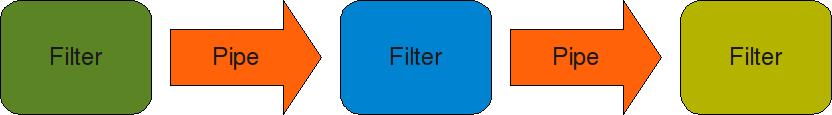
\includegraphics[scale=0.7]{pics/pipesFilter3.png}
	\caption[Pipes and Filter]{
	\textbf{pipesFilter.}
	something}
	\end{center}
	\label{fig:pipesFilter}
\end{figure}

Die zu annotierende Sequenz wird schrittweise durch verschiedene \first{Filter}
bearbeitet. Jeder Filter, der in der Pipeline vorhanden ist, wird dabei das
entgültige Ergebnis der Annotation durch seine spezifischen Ergebnisse
erweitern.

Der Input eines Filters besteht dabei zum einen aus der zu
annotierenden Sequenz selbst, zum anderen aus einem zentralen Datenobjekt, in
dem alle gewonnenen Ergebnisse abgespeichert werden.
Ein Filter kann dabei auch auf die Ergebnisse eines anderen
Filters angewiesen sein. Die Reihenfolge der Filter innerhalb der Pipeline wird
somit durch die spezifischen \first{execution preconditions}
\footnote{\todo{execution precondition}} aller Filter festgelegt.
\index{Filter}
\index{execution precondition}

Es ist davon auszugehen, dass die Ausführung einzelner Filter mitunter sehr
zeitintensiv sein wird. Ausserdem soll Nutzen aus dem im Institut installierten
\first{LSF} gezogen werden. Daher wird eine rein sequenzielle Abfolge der
Filter, wie es das Entwursmuster suggeriert, vermieden werden.
Stattdessen kann die Ausführung einzelner Filter parallel erfolgen.
Sind zu einem Zeitpunkt die execution preconditions mehrerer Filter erfüllt,
werden alle sofort zur Ausführung gebracht.
\index{Platform LSF}

Die Pipeline soll möglichst leicht konfigurierbar sein und sich an
individuelle Bedürfnisse anpassen lassen.
Vor diesem Hintergrund soll die Pipeline die veränderbaren Steps und das
statische \enquote{Ausführungsgerüst} vollständig entkoppeln. Beim Starten der
Pipeline soll diese an einem bestimmten Ort (lokales Verzeichnis oder
entferntes Repository) nach vorhandenen Steps suchen und diese in der Pipeline
installieren.

Die \name{Filter} des \name{pipes and filters} pattern sind somit aus der
eigentlichen Anwendung herrausgelöst. Sie sind über eine generische
Schnittstelle repräsentiert, deren Implementierung zur Kompilierzeit nicht
bekannt ist.

\begin{figure}[htbp]
	\begin{center}
		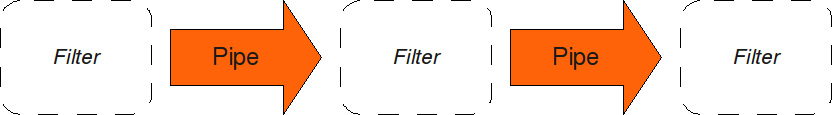
\includegraphics[scale=0.7]{pics/pipesFilter21.png}
	\caption[Pipes and Filter 21]{
	\textbf{pipesFilter 21.}
	something}
	\end{center}
	\label{fig:pipesFilter21}
\end{figure}

Die Pipeline teilt sich so in zwei Teilkomponenten:
Die \enquote{dynamischen Stepss} und das \enquote{statisches Ausfürhungsgerüst}.
Diese Anordnung legt eine weitere Abstraktionsebene nahe, nämlich das
\first{Client-Server-Modell}.
\footnote{\todo{Client-Server-Modell}}
\index{Client-Server-Modell}

\subsection{Client-Server-Modell}
Die \first{Pipes} des \name{pipes and filters} Pattern werden zu einem
\first{Server} zusammengefasst und bilden das {statische Ausführungsgerüst}.
Ein \first{Client} ist ein \first{Filter} des \name{pipes and filters} Pattern.
Die einzelnen Clients sind dynamisch und somit nicht Teil der
statischen Kernanwenung.
\index{Filter}
\index{Step}
\index{Client}
Es können sich beliebig viele Clients am Server anmelden, wodurch die
eigentliche Pipeline aufgebaut wird.
\todo{hmmhmm}

\subsubsection{Server}
Die Anforderungen an den Server gliedern sich in zwei Teilbereiche:
\begin{description}
\item[Organisation und Synchronisation der Client Ausführung]
Die Ausfürhrung der angemeldeten Steps kann sequenziell oder
parallel erfolgen, je nachdem, welche \first{execution preconditions} für den
jeweiligen Step erforderlich sind und ob die zur Ausführung benötigten Daten eventuell erst
durch einen anderen Step bereitgestellt werden müssen. Vor der eigentlichen
Ausführung wird der Server somit zum einen die \name{execution preconditions}
prüfen, zum anderen, ob der Step überhaupt zur Ausführung
gebracht werden muss, oder ob die zu erwartenden Ergebnisse bereits in selber
oder in anderer Form vorhanden sind.
\item[Datenverwaltung] Die Ergebnisse der einzelnen Steps werden zentral durch
den Server verwaltet.
Zum einen synchronisiert der Server die Zugriffe auf die Daten, zum anderen
werden diese persistiert, um bei einer gewollten oder ungewollten Unterbrechung
der Pipeline Datenverlust zu verhindern.
\end{description}

\subsubsection{Client}
Auf der Clientseite stehen die einzelnen \first{Filter} der Pipeline, im
folgenden \first{Steps} genannt \todo{hmmm}. Jeder Step soll technisch
gesehen einem oder mehreren OSGi-Bundles entsprechen.
\index{Step}
\index{Filter}
\index{Client}
\index{Bundle}
\index{OSGi-Bundle}
Wird das Bundle durch das OSGi-Framework gestartet, soll sich der Step am Server
anmelden. Der Step stellt dabei entsprechende \name{call-back-Methoden} für die
eigentliche Ausführung, Überprüfung der \name{execution preconditions} und
Ähnlichem bereit.
\index{Server}
\index{OSGi Framework}
\index{call back method}
Wann diese Methoden aufgerufen werden, obliegt so allein
dem Server.
Als Prameter der call back methoden wird die Sequenz, sowie das zentrale
Datenobjekt, im Folgenden \first{Data bean} \todo{hmmm} genannt,
übergeben.

\begin{figure}[htbp]
	\begin{center}
		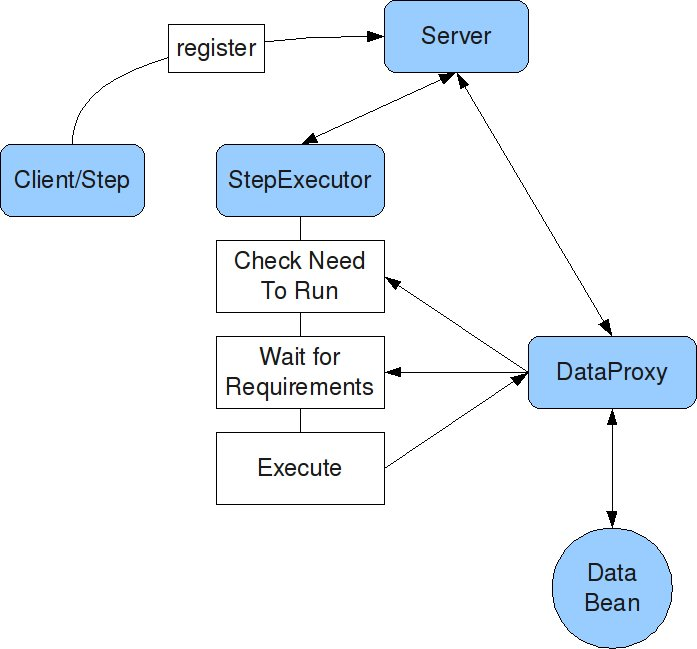
\includegraphics[scale=0.6]{pics/programOrganisationOverview3ScaledWithAlpha.jpg}
	\caption[Design 1]{
	\textbf{Design 1.}
	something. \todo{Teilung von Server hier noch nicht erwähnt. Evtl. Teil der
	Umstzung}}
	\end{center}
	\label{fig:programOrganisationOverview3ScaledWithAlpha}
\end{figure}